\chapter{Implementation, Performance Analysis and Optimization}
\label{Chapter5}
\lhead{Chapter 5. \emph{Implementation, Performance Analysis, and Optimization}}

\section{Algorithmic Overview and Pseudocode}

% \swb{The following paragraph should go in Section 4.2. Only write about the algorithm here.}
In this section, we will elaborate on the logical flow of the program for our method. For complete code, refer to Appendix \ref{AppendixB}. 
\subsection{Important Helper Functions}
\textbf{Screening Factor Array}: This function computes the product of the screening factor array defined in Eq.~(\ref{eq:N2D-ScreenFunction}) and the B-spline coefficient array defined in Eq.~(\ref{eq:bsplineArray}). This array can be precomputed and stored in memory prior to running the simulation, allowing it to be reused throughout the runs.
\lstinputlisting[language=C]{CodeFiles/screenfunction.c}

\textbf{Implementing \ac{MIC}}: This function calculates the distance between two atoms using the \aclu{MIC} (\ac{MIC}) for system with 2D periodicity.
\lstinputlisting[language=C]{CodeFiles/mic.c}

\subsection{Functions to Compute Energies}
\textbf{Real Space Energy}: The loops in this function computes the total real space energy. 
\lstinputlisting[language=C]{CodeFiles/real.c}

\textbf{Reciprocal Space Energy with Particle Mesh Adaptation}: The loops in this function computes the total reciprocal space energy. 
\lstinputlisting[language=C]{CodeFiles/reci.c}

\section{Analysis of Baseline Program}

After implementing the new 2D Ewald summation algorithm, the subsequent objective was to identify performance bottlenecks in the program, as the next critical step in guiding further optimization efforts. Intel\textsuperscript{\textregistered} VTune\texttrademark{} Profiler was used for this purpose. VTune supports a wide range of analysis types, including Hotspots, Microarchitecture Exploration, Threading, Memory Access, and Platform analysis. With support for multiple programming languages and parallelization frameworks like OpenMP and MPI, VTune improves application speed, scalability, and hardware efficiency across diverse Intel architectures. 

The Hotspot analysis is particularly useful in the early development process of an application as it helps pinpoint the sections of code where the CPU spends the most time, guiding the optimization efforts for maximum performance gains. In the Bottom-up window, detailed performance data is grouped by function and sorted by CPU time. Functions with high CPU time should be prioritized for optimization.

% \swb{Write a few more lines justifying our choice with VTune. Also, list a few different program analyses that VTune supports. Tell readers what is analysed in hotspot analysis and what is the expected output.}

% \swb{It seems we need to briefly describe the implementation before we talk about profiling it.}

Hotspot analysis of the baseline program was performed to identify computational bottlenecks. The results in Fig.~(\ref{fig:result1vtune}), indicate that the real-space component accounts for approximately 60-65\% of the total CPU time. The most expensive function was \texttt{dist}, responsible for inter-particle distance calculations, consuming around 25\% of the execution time. This cost is compounded by repeated calls to the \texttt{\_\_erfc} function, contributing approximately 20\% of the total runtime. These findings highlight the need to optimize the real-space calculations, particularly the error function evaluation, to improve overall performance.

While both \texttt{dist} and \texttt{\_\_erfc} are major contributors to the CPU Time, the \texttt{dist} function offers limited scope for optimization due to the straightforward nature of the algorithm. Therefore, the focus shifts to the \texttt{\_\_erfc} function from \texttt{libm}, the standard math library in the GNU C Library. Using a faster or approximate version of the error function could help reduce execution time and improve performance.

% \swb{What is \texttt{libm}?}

% \begin{figure}[htbp]
\begin{figure}[H]
    \centering
    \begin{minipage}{0.7\textwidth}
        \fbox{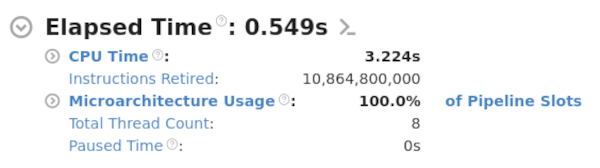
\includegraphics[width=\linewidth]{images/VTuneInitialTime.png}}
    \end{minipage}%
    \begin{minipage}{0.3\textwidth}
        \caption{Execution time details for baseline program.}
    \end{minipage}
\end{figure}
% \begin{figure}[htbp]
\begin{figure}[h]
    \centering
    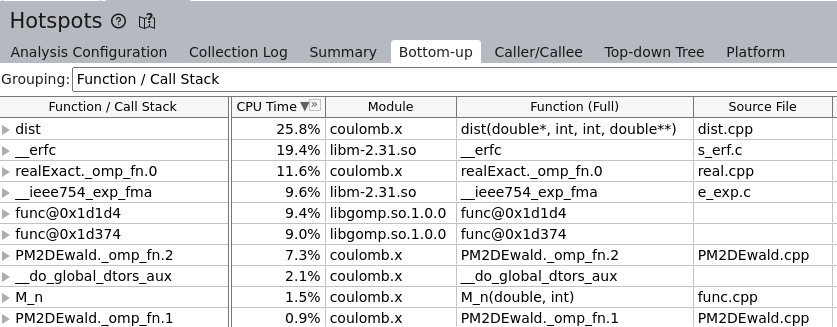
\includegraphics[width = \linewidth]{images/VTuneInitialHotspot.png}
    \caption{Hotspot analysis of the baseline Ewald summation implementation, as reported by Intel VTune Profiler. A significant portion of total CPU time is concentrated in the \textit{dist} function (25.8\%), the standard math library's \textit{\_\_erfc} function (19.4\%).}
    \label{fig:result1vtune}
\end{figure}

\section{Polynomial Interpolation Optimization}
\subsection{Polynomial Interpolation of Error Function}
As deduced in the previous section, a significant portion of the program’s execution time was consumed by calls to the \verb|std::erfc| function. To reduce the computational cost associated with evaluating the complementary error function \(\operatorname{erfc}(x)\) in the real-space part of the Ewald summation, a polynomial interpolation approach was adopted. This technique is outlined in \textit{Handbook of Mathematical Functions by Abramowitz and Stegun}~\cite{abramowitz1965handbook}. The expression used is
\begin{equation}  
    erf(x) = 1 - (a_1 t + a_2 t^2 + a_3 t^3 + a_4 t^4 + a_5 t^5) e^{-x^2} + \epsilon(x)
\end{equation}
\[
    t = \frac{1}{1 + px}, \quad |\epsilon(x)| \leq 1.5 \times 10^{-7},
\]
\[
p = 0.3275911, \\
a_1 = 0.254829592, \\
a_2 = -0.284496736,
\]
\[
a_3 = 1.421413741, \\
a_4 = -1.453152027, \\
a_5 = 1.061405429.
\]
The polynomial was subsequently adapted as a replacement for the standard $\operatorname{erfc}(x)$ function in the real-space evaluation. This approach is advantageous because $\operatorname{erfc}(x)$ is computationally more expensive than $\operatorname{exp}(x)$. The evaluation of $\operatorname{erfc}(x)$ requires complex numerical approximations to compute an integral that does not have a simple closed form. In contrast, $\operatorname{exp}(x)$ is simpler and optimized, which makes it significantly faster to compute.

\subsection{Efficiency and Accuracy}
In order to assess the efficiency of the interpolation-based approach, a series of computations were performed. The number of ions in the system was varied while keeping the box side constant at 25 \AA. 

As shown in the Fig.~(\ref{fig:realspaceopt}), this numerical optimization resulted in a significant improvement in performance. On an average, the interpolation method achieved a $15\%$ reduction in runtime, showing improved scalability and efficiency, especially for larger system sizes. This speed-up was achieved without compromising numerical accuracy; the maximum relative error in the real space energies was less than $10^{-5}$, which is well within the acceptable bounds for energy calculations in molecular simulations.
\begin{figure}[H]
    \centering
    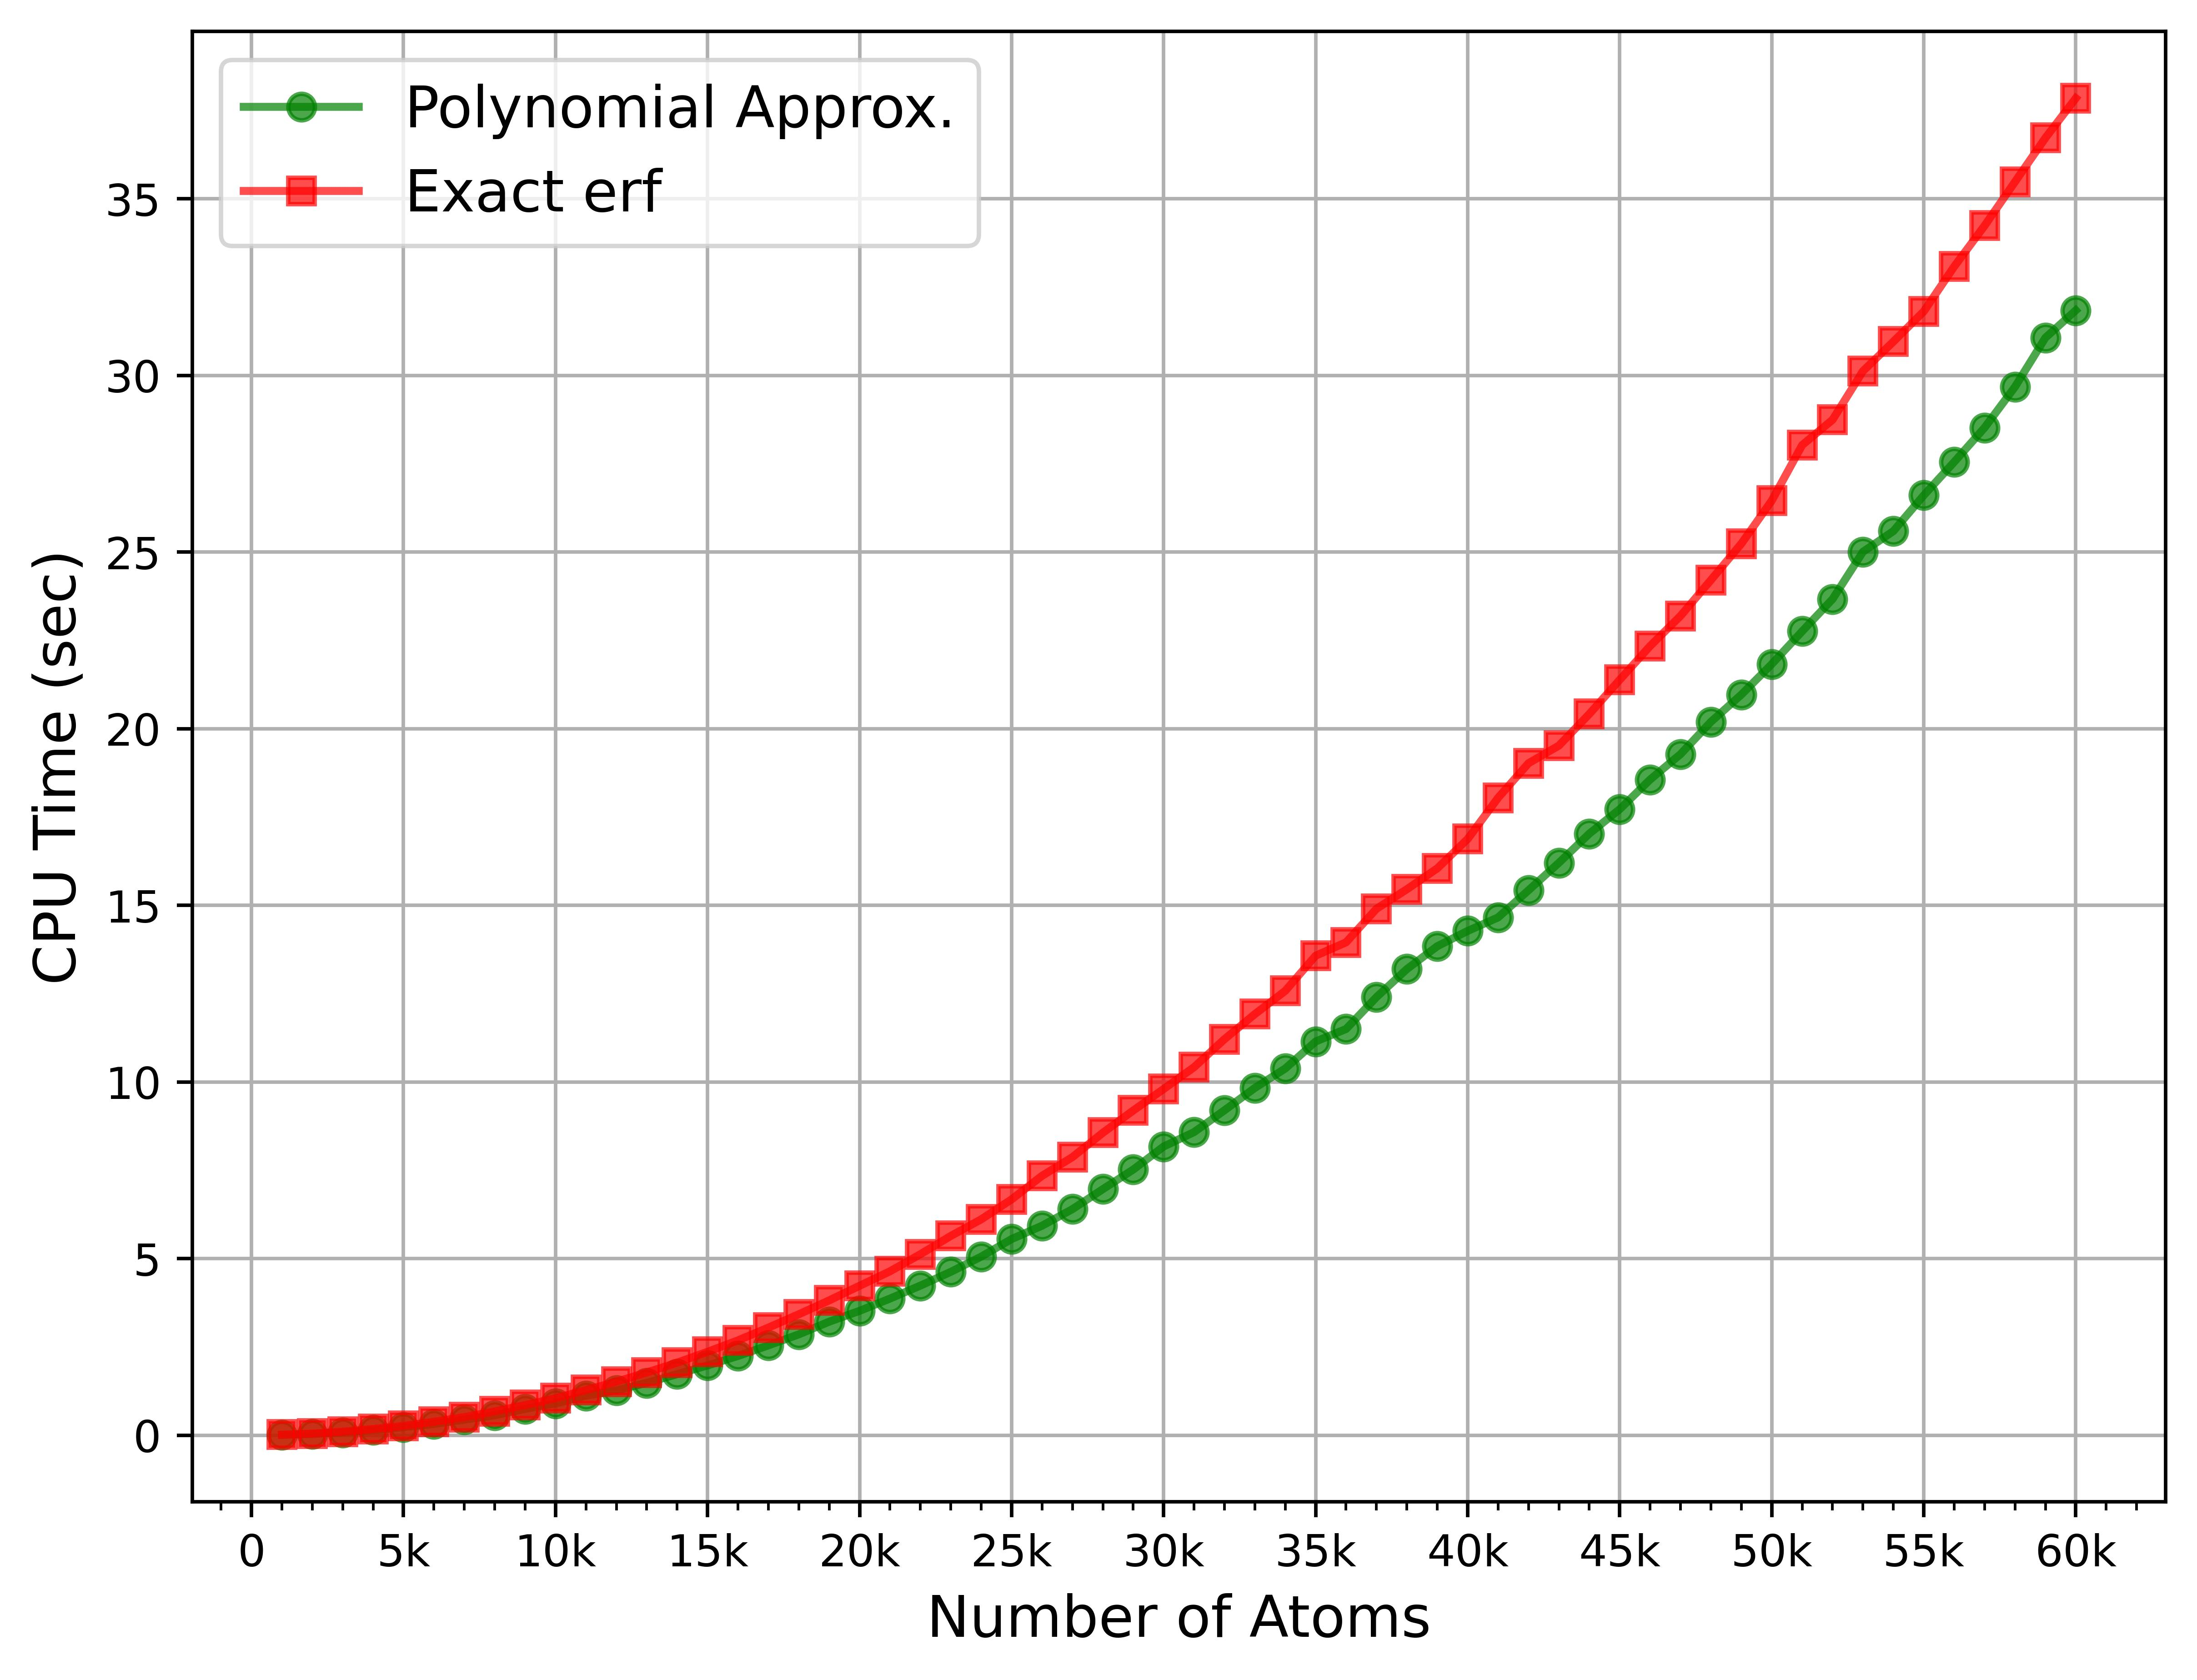
\includegraphics[width=0.75\linewidth]{images/realspaceopt.jpg}
    \caption{Comparison of CPU runtime between the polynomial approximation and exact error function evaluation to compute real space energy as a function of the number of atoms. The side length of the simulation box was fixed at 25 \AA. The polynomial approximation method demonstrates a consistent speed-up of approximately $15\%$ across all system sizes, while maintaining relative errors under $10^{-5}$}
    \label{fig:realspaceopt}
\end{figure}

\section{Code-Level Optimizations}
\subsection{Array Flattening}
In the implementation, data involving multiple dimensions must be stored in several parts of the program, such as atom positions and charge spreading array for the SPME. While multidimensional arrays are a natural choice for such data, they have drawbacks. 

Dynamically allocated multidimensional arrays often lead to scattered memory layouts and multiple pointer dereferences. This results in poor cache performance and added complexity in memory management. 
To address this, a one-dimensional array was used to represent the multidimensional structure. For an array with rank $d$ and dimensions $n_1\times \ldots \times n_d$, an element at ($i_1\times \ldots \times i_d$) maps to:
\begin{flalign*}
    i_d + n_d \cdot \left( i_{d-1} + n_{d-1} \cdot \left( \ldots + n_2 \cdot i_1 \right)\right)
\end{flalign*}
This approach reduced overhead, improved memory locality, and allowed faster access through direct indexing. %%In the paper we would want to elaborate this...
\subsection{Vectorization}
Vectorization enables the simultaneous processing of multiple data elements using a single instruction. This approach significantly improves both the speed and efficiency of computations. It is a fundamental technique in high-performance numerical computing, scientific simulations, graphics, and machine learning, as it leverages the SIMD (Single Instruction Multiple Data)~\cite{hennessy2017computer} capabilities present in modern processors.

In this work, the program has been compiled using the flags \texttt{-O3}, \texttt{-mavx2}, \texttt{-march=native}, \texttt{-ftree-vectorize}, and \texttt{-ftree-vectorizer-verbose=1}. The \texttt{-O3} flag enables aggressive optimization, including automatic vectorization of loops. The \texttt{-mavx2} flag ensures that the generated code utilizes AVX2 instructions, which operate on 256-bit registers. This allows the simultaneous processing of 8 single-precision floating-point numbers or 4 double-precision floating-point numbers, thereby greatly accelerating loops and computation-intensive sections of the code.


\section{Profiling of Optimized Program}
% \section{Performance of Optimized Implementation}
Following the improvements, hotspot analysis of the optimized implementation Fig.~(\ref{fig:resultVTuneFinal}), shows a notable shift in the computational profile. The \texttt{\_\_erfc} function no longer appears among the major hotspots. The primary contributors to CPU time are now \texttt{dist} (35.4\%) and \texttt{real\_omp\_fn.0} (23.2\%), both associated with real-space computations.  %%%For the paper, could we give a reason that paralellization can improve this bottleneck. 
% Detailed performance improvements are presented in the \textit{Numerical Analysis} section of the thesis.
\begin{figure}[htbp]
% \begin{figure}[]
    \centering
    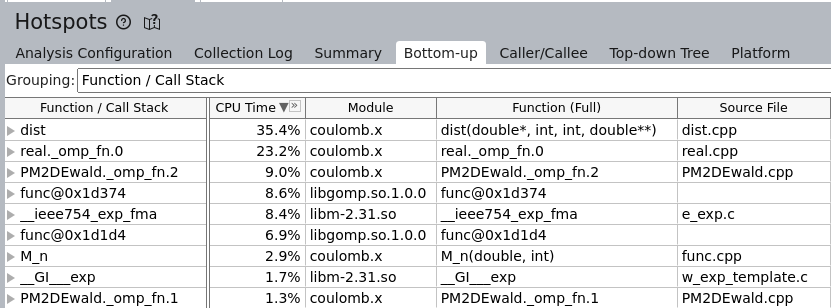
\includegraphics[width = \linewidth]{images/VTuneFinalHotSpots.png}
    \caption{Hotspot analysis of the optimized Ewald summation implementation, using a polynomial interpolation for the error function. The overall CPU time distribution indicates improved efficiency in the real-space term.}
    \label{fig:resultVTuneFinal}
\end{figure}
\begin{figure}[h]
% \begin{figure}[]
    \centering
    \begin{minipage}{0.7\textwidth}
        \fbox{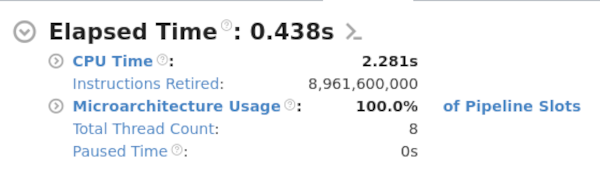
\includegraphics[width=\linewidth]{images/VTuneFinalTime.png}}
    \end{minipage}%
    \begin{minipage}{0.3\textwidth}
        \caption{Execution time details for improved program.}
    \end{minipage}
\end{figure}

\section{Parallelization}
Parallel programming can have an enormous impact on the performance and scalability of computational applications~\cite{pacheco2011introduction}. The motivation for parallelizing code is to reduce its execution time, enabling it to run faster on modern multiprocessor systems. In this context, the Ewald summation algorithm is crucial, as it is computationally intensive. Depending on the specific component of the calculation, its computational complexity ranges from $O(N^2)$ to $O(NlogN)$, making it essential to accelerate through parallel techniques. Efficient parallelization is critical for simulating long-range interactions in order to study large-scale systems.

\subsection{OpenMP}
In the Ewald summation method, a significant portion of the execution time is consumed by for loops. These loops are particularly well-suited for parallelization using OpenMP~\cite{dagum1998openmp}, a shared-memory parallel programming model that efficiently distributes computational workloads across multiple threads, thereby enhancing overall performance.

% \swb{Cite OpenMP.}

OpenMP facilitates incremental parallelization of existing sequential code with minimal modifications. Its accessibility and simplicity make it especially advantageous, as it does not require specialized hardware such as supercomputers. Instead, it can yield substantial performance improvements even on standard personal computers equipped with multi-core processors.

OpenMP utilizes \verb|#pragma|  directives, which are combined with directive specifications and optional clauses. An OpenMP directive begins with \verb|#pragma omp|, followed by a specific directive keyword. 
By default, OpenMP creates a number of threads that is typically equal to the number of CPU cores available. However, this can also be modified via \verb|omp_set_num_threads()| function. For instance, the parallelization of a for loop is expressed as follows:
\lstinputlisting[language=C]{CodeFiles/forloop.c}

% \swb{Did you mention how many threads are created by default?}

\subsection{Ensuring Correctness in Loop-Carried Dependencies}
\textbf{Reduction:} The \verb|reduction| clause is used to safely accumulate the result of a shared variable such as the real or the reciprocal energies. Each thread maintains a private copy of the reduction variable, and they automatically combine that at the end of the parallel region using the specified reduction operator. An example of its application in the reciprocal space energy calculation is shown below
\lstinputlisting[language=C]{CodeFiles/reduction.c}

\textbf{Race condition during charge spreading:} A naïve approach that assigns one thread to map each charge onto the grid can lead to synchronization issues when multiple threads attempt to update the same grid point. During the computation of the charge spreading array $Q$, overlapping interpolation regions may cause several threads to modify the same grid location at the same time, resulting in a race condition and potentially incorrect values. To handle this, the \verb|atomic update| clause in OpenMP was used to ensure that updates are performed atomically, thereby preventing simultaneous read and write operations by different threads.
\lstinputlisting[language=C]{CodeFiles/atomic.c}

\textbf{Nested loops:} To parallelize the independent nested loops involved in the reciprocal space summation over the three-dimensional grids, the \texttt{collapse(3)} clause is employed. This directive flattens the nested loops into a single iteration space, thereby enhancing load balancing and facilitating uniform distribution of the computational workload across threads.
\lstinputlisting[language=C]{CodeFiles/collapse.c}
% \clearpage
\subsection{Performance Evaluation}
To evaluate the effectiveness of OpenMP-based parallelization, a series of calculations were performed across different system sizes. The execution times were recorded by varying the number of OpenMP threads from 1 to 23, examining the scalability of the program. 
\begin{figure}[htbp]
    \centering
    \subfigure[Total simulation time for different thread counts for direct Ewald summation for our new formulation.]{%
        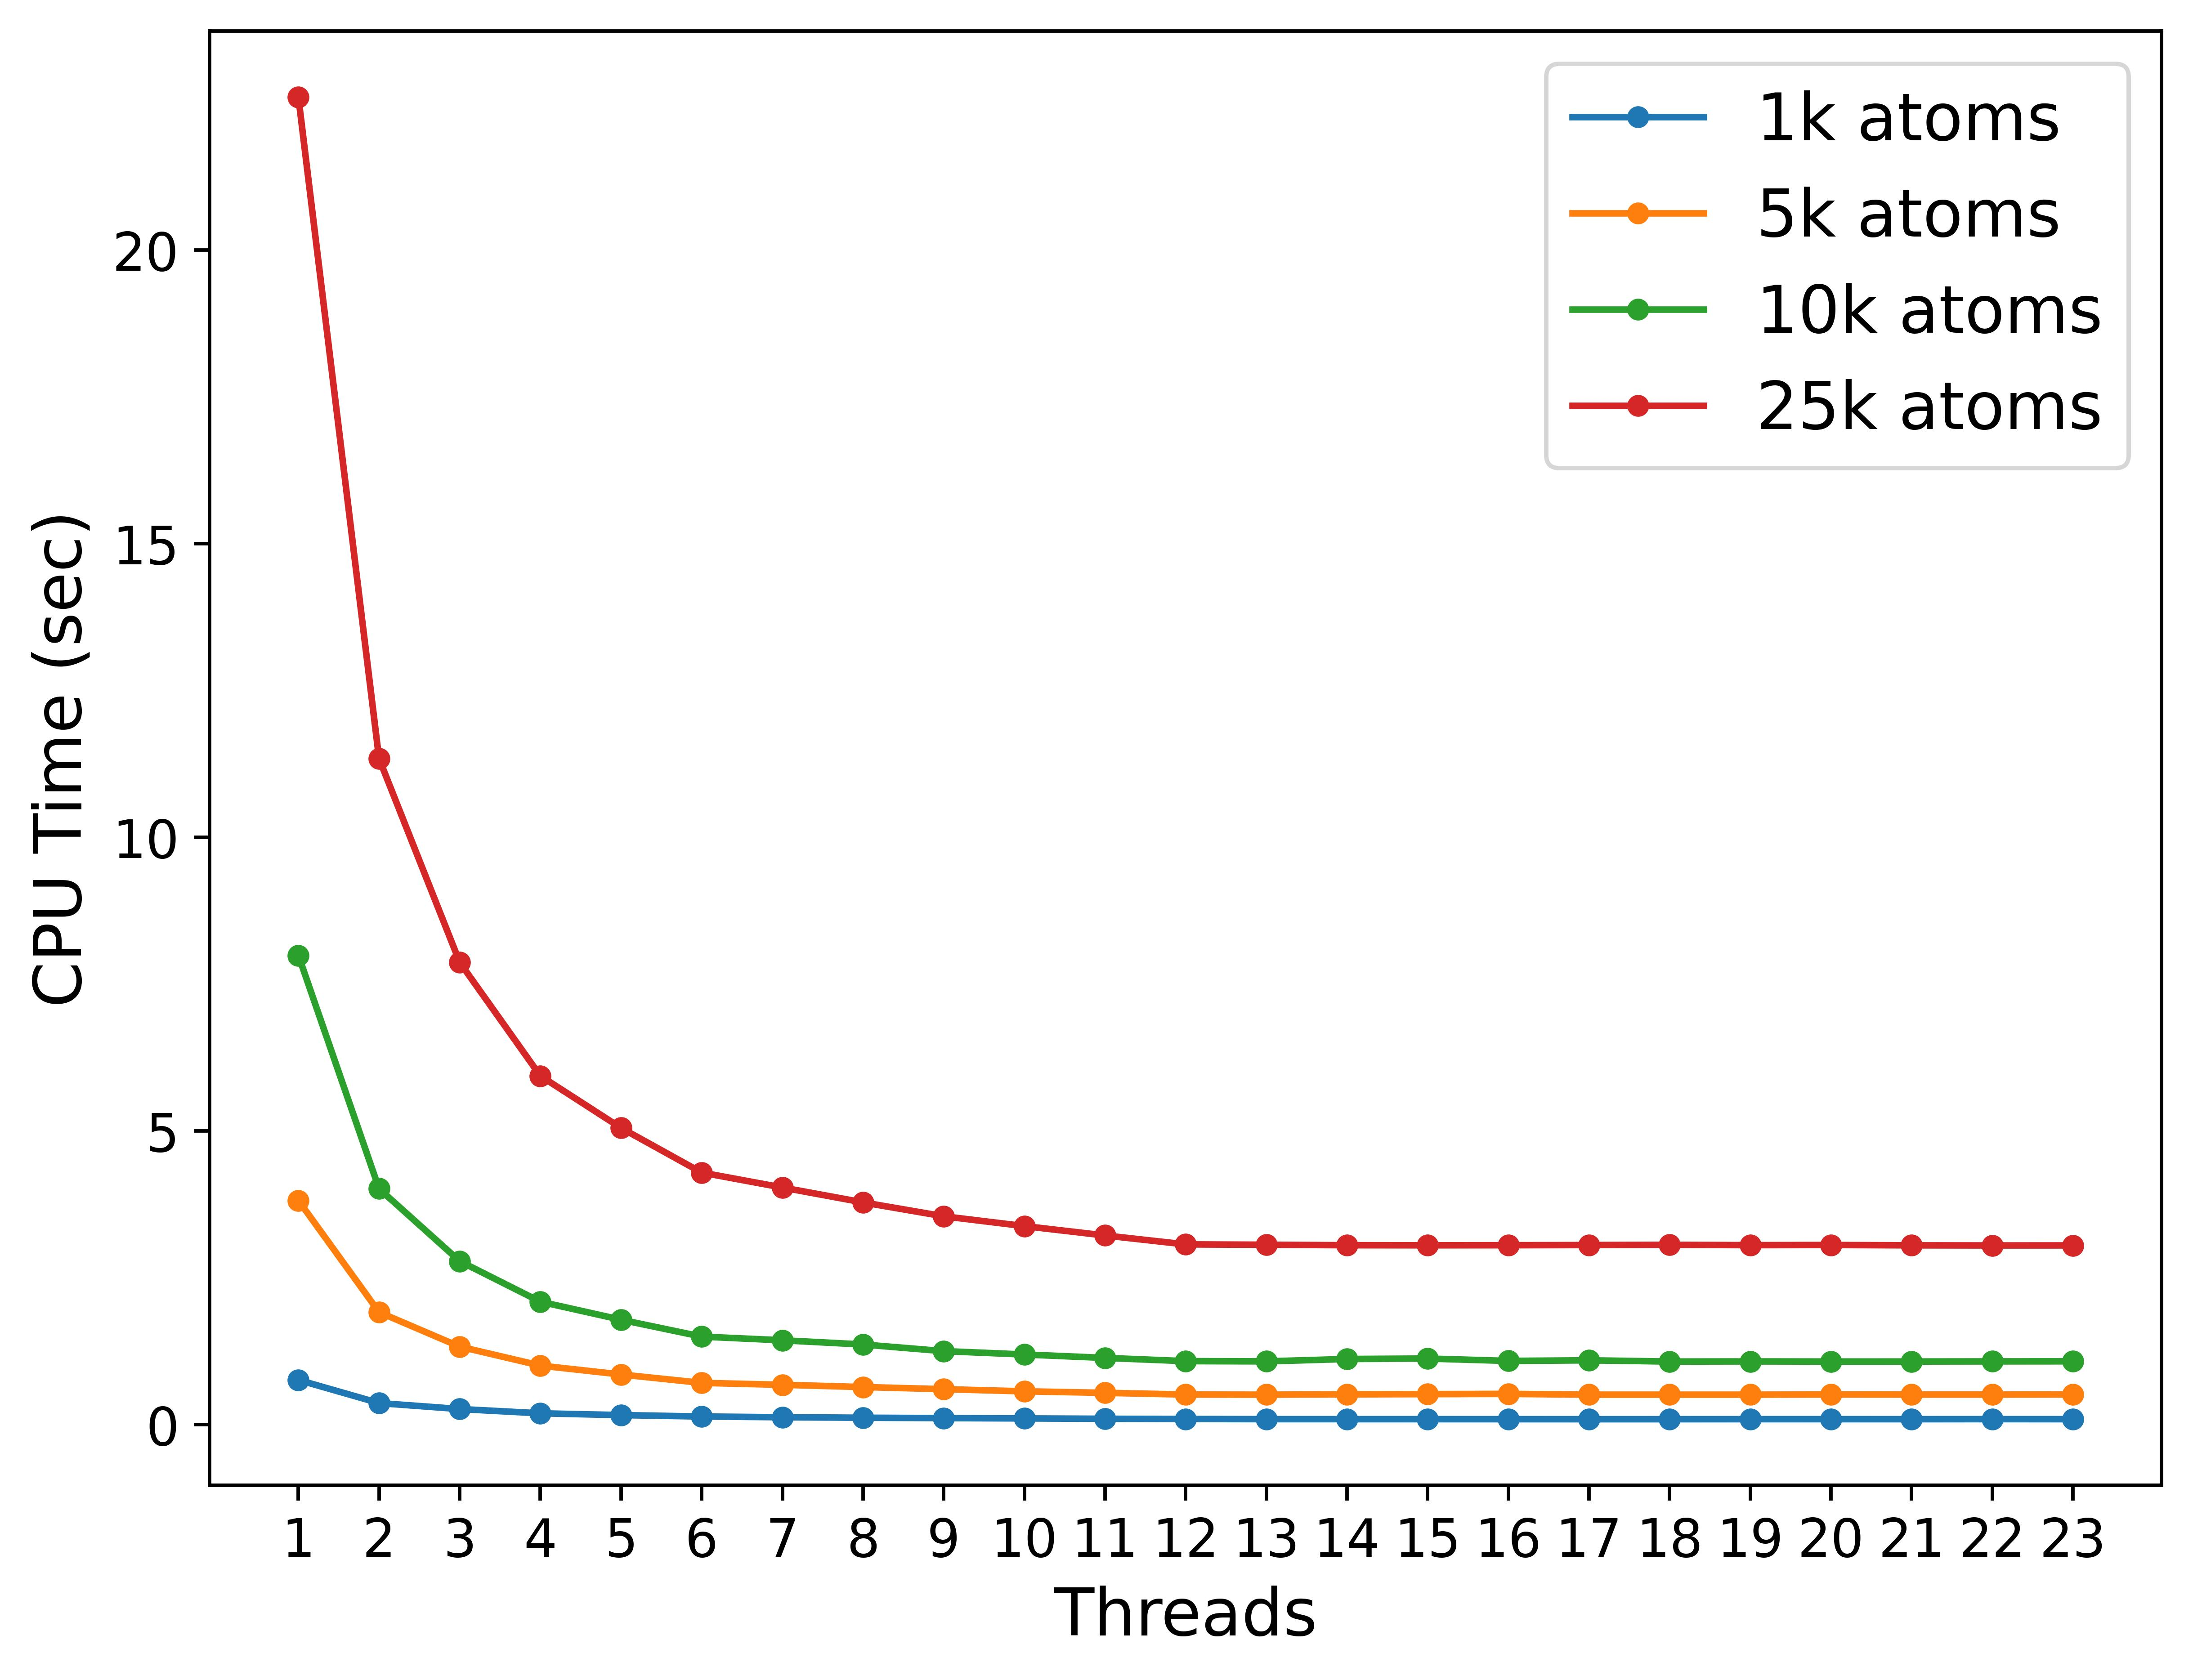
\includegraphics[width=0.45\textwidth]{images/threadstimetotal.jpg}
        \label{fig:thread-a}
    }
    \hfill
    \subfigure[Total simulation time for new method with particle mesh interpolation (grid: $64 \times 64 \times 512$, order: 8) across different thread counts.]{%
        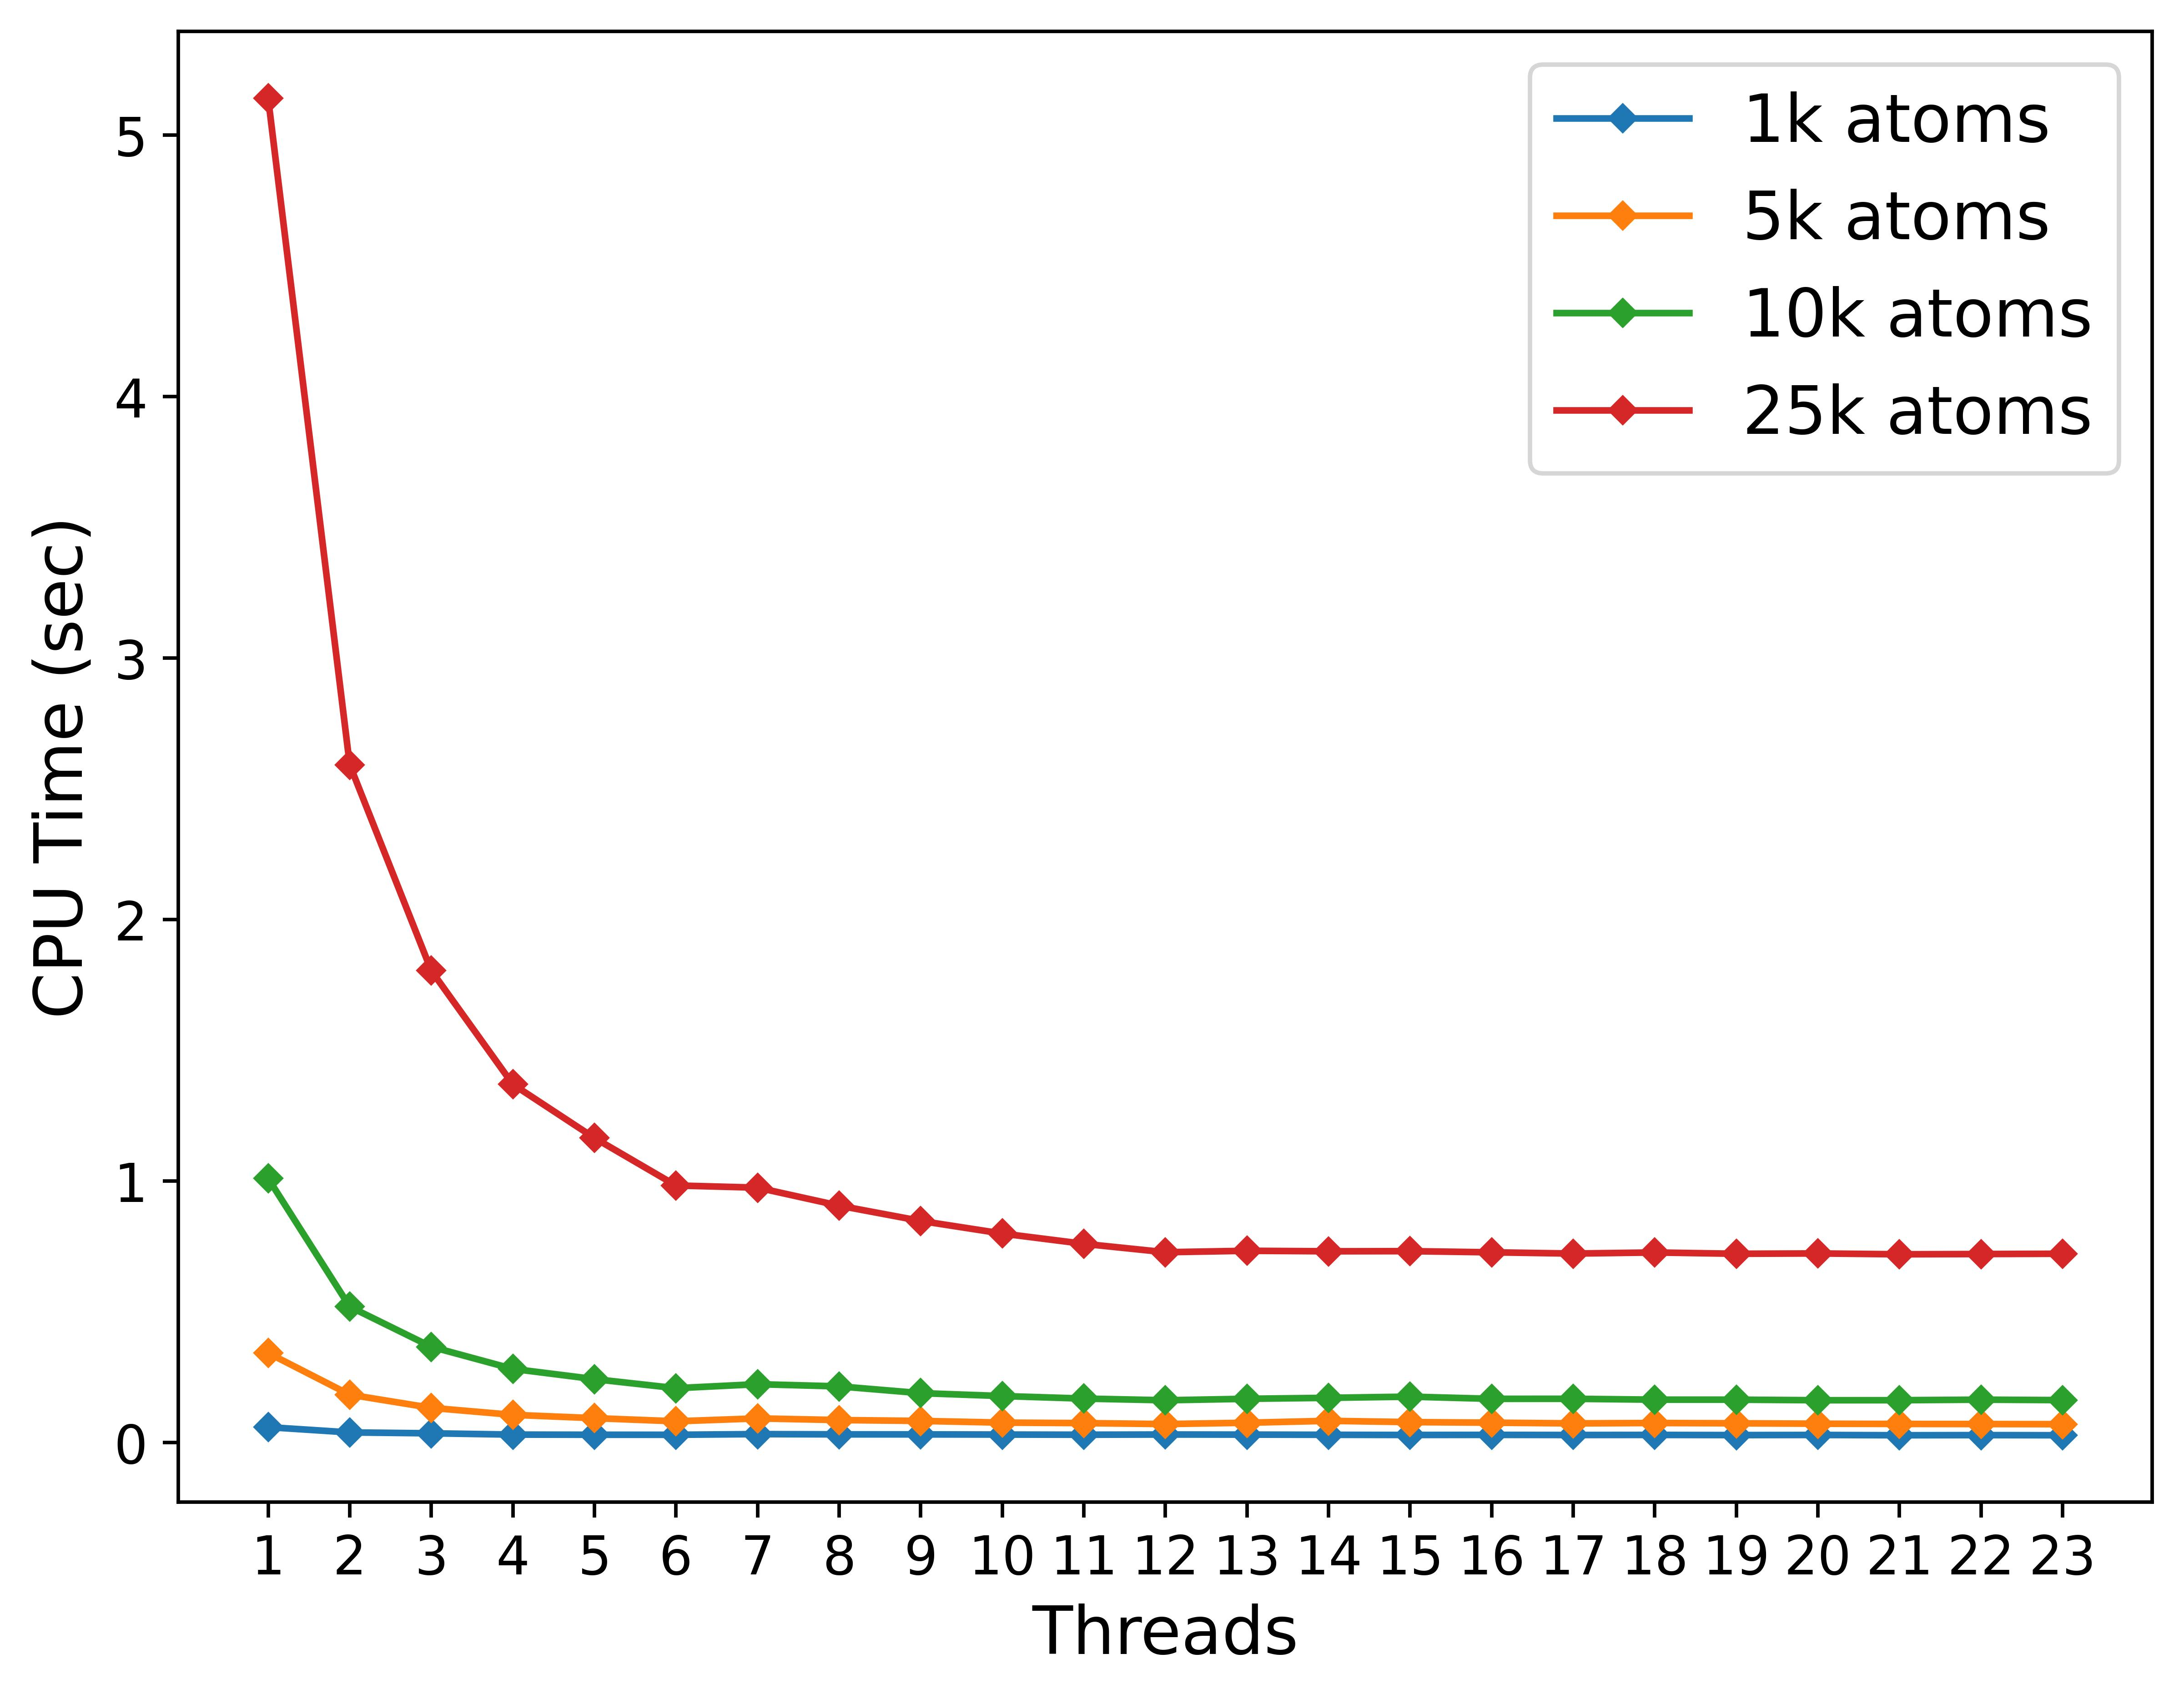
\includegraphics[width=0.45\textwidth]{images/threadstimeSPMEtotal.jpg}
        \label{fig:thread-b}
    }
    \caption{Comparison of total simulation time for new formulation across different thread counts for (a) direct Ewald summation and (b) particle mesh interpolation. Performance improves significantly with multithreading, particularly up to the number of physical cores available.}
    \label{fig:threading}
\end{figure}

The results demonstrate a significant reduction in the execution times with increasing threads, up to 12, which corresponds to the number of physical CPU cores available on the system. Beyond this point, the performance improvement begins to plateau. This behaviour shows the potential of parallelization within the bounds of the available hardware, and further improvements may require more advanced hardware.